\documentclass[tikz]{standalone}
\usepackage{tikz}
\begin{document}    
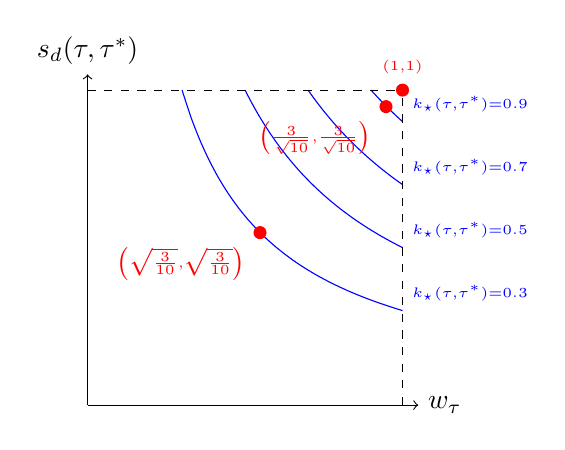
\begin{tikzpicture}
  \draw[->] (0, 0) -- (4.2, 0) node[right] {$w_\tau$};
  \draw[->] (0, 0) -- (0, 4.2) node[above] {$s_d(\tau,\tau^*)$};
  \draw[scale=4, domain=0.9:1, smooth, variable=\x, blue] plot ({\x}, {0.9/\x}) node[above right]{$\scriptscriptstyle{k_\star(\tau,\tau^*)=0.9}$};
  \draw[scale=4, domain=0.7:1, smooth, variable=\x, blue] plot ({\x}, {0.7/\x}) node[above right]{$\scriptscriptstyle k_\star(\tau,\tau^*)=0.7$};
  \draw[scale=4, domain=0.5:1, smooth, variable=\x, blue] plot ({\x}, {0.5/\x}) node[above right]{$\scriptscriptstyle k_\star(\tau,\tau^*)=0.5$};
  \draw[scale=4, domain=0.3:1, smooth, variable=\x, blue] plot ({\x}, {0.3/\x}) node[above right]{$\scriptscriptstyle k_\star(\tau,\tau^*)=0.3$};
  %\draw[scale=4, domain=0.1:1, smooth, variable=\x, blue] plot ({\x}, {0.1/\x}) node[above right]{$\scriptscriptstyle xy=0.1$};
  \draw[dashed] (0,4) -- (4,4);
  \draw[dashed] (4,0) -- (4,4);
  
  \node[shape=circle,fill=red, scale=0.5,label=above:{$\color{red} \scriptscriptstyle (1,1)$}] at (4,4)  {};
  \node[shape=circle,fill=red, scale=0.5,label=below left:{$\color{red} \scriptscriptstyle \left(\sqrt{\frac{3}{10}},\sqrt{\frac{3}{10}}\right)$}] at (2.19,2.19)  {};
  \node[shape=circle,fill=red, scale=0.5,label=below left:{$\color{red} \scriptscriptstyle \left(\frac{3}{\sqrt{10}},\frac{3}{\sqrt{10}}\right)$}] at (3.79,3.79)  {};
\end{tikzpicture}
\end{document}

